\documentclass[../../generative_classifiers.tex]{subfiles}
\begin{document}
\graphicspath{{figures/}{lectures/05_generative_gda/figures/}}
\section{Generative Classifiers (GDA)}
\begin{frame}[plain]
  \vfill\begin{center}{\Huge \textcolor{blue}{Generative Classifiers (GDA)}}\end{center}\vfill
\end{frame}
\begin{frame}[fragile]{Generative Classifiers}

In this lecture, we are going to look at generative classifiers and their applications.
\vspace{0.2cm}

We will continue using the Iris dataset for classification. The task is to classify subspecies of Iris flowers based on their measurements:

\begin{lstlisting}
import numpy as np; np.set_printoptions(precision=2)
import pandas as pd; pd.options.display.float_format = "{:,.2f}".format
import warnings; warnings.filterwarnings('ignore')
from sklearn import datasets

iris = datasets.load_iris(as_frame=True)
iris_X, iris_y = iris.data, iris.target
pd.concat([iris_X, iris_y], axis=1).sample(5, random_state=0)
\end{lstlisting}

\begin{figure}[h]
    \centering
    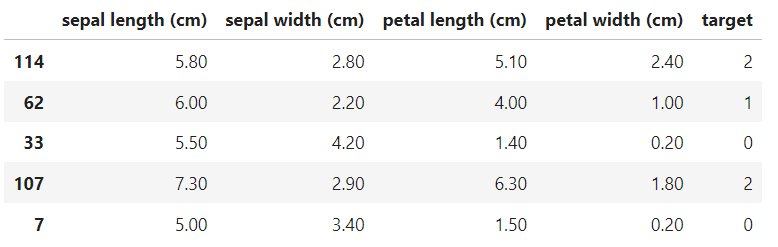
\includegraphics[width=0.52\textwidth]{picture_1.png}  % Ajusta el nombre y la ruta de la imagen
\end{figure}
\end{frame}


\begin{frame}[fragile]{Generative Classifiers}
If we only consider the first two feature columns, we can visualize the dataset in 2D.
\begin{lstlisting}
import matplotlib.pyplot as plt
plt.rcParams.update({ "figure.figsize": [6, 2], "figure.dpi": 150, "text.usetex": True, "font.family": "Helvetica"})

# create 2d version of dataset
X = iris_X.to_numpy()[:,:2]
x_min, x_max = X[:, 0].min() - .5, X[:, 0].max() + .5
y_min, y_max = X[:, 1].min() - .5, X[:, 1].max() + .5

# Plot also the training points
p1 = plt.scatter(X[:, 0], X[:, 1], c=iris_y, edgecolor='k', s=60, cmap=plt.cm.Paired)
plt.xlabel('Sepal Length (cm)'); plt.ylabel('Sepal Width (cm)')
plt.legend(handles=p1.legend_elements()[0], labels=['Setosa', 'Versicolour', 'Virginica'], loc='lower right');
\end{lstlisting}

\end{frame}

\begin{frame}[fragile]{Generative Classifiers}

\begin{figure}[h]
    \centering
    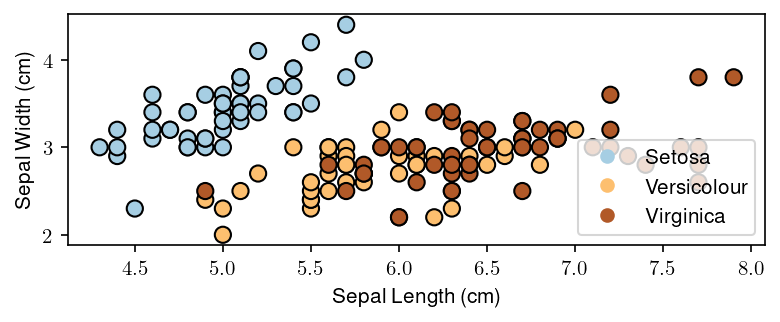
\includegraphics[width=1\textwidth]{picture_2.png}  % Ajusta el nombre y la ruta de la imagen
\end{figure}

\end{frame}


\begin{frame}[fragile]{Review: Supervised Learning Models}

A supervised learning model can be seen as directly predicting a one-hot embedding of the target class:

$$
\underbrace{\left[ 
\begin{array}{c}
x_1 \\
x_2 \\
x_3 \\
x_4 \\
\end{array}
\right]}_\text{input}
{\to}\text{model $f_\theta(x)$}{\to}
\underbrace{\left[ 
\begin{array}{c}
0 \\
1 \\
0 \\
\end{array}
\right]}_\text{output}
$$

In this example, the $f_\theta(x)$ predicts the second class for input $x$.

\end{frame}


\begin{frame}[fragile]{Review: Probabilistic Models}

A probabilistic model outputs a vector of class probabilities

$$
\underbrace{\left[ 
\begin{array}{c}
x_1 \\
x_2 \\
x_3 \\
x_4 \\
\end{array}
\right]}_\text{input}
{\to}\text{model $P_\theta(y|x)$}{\to}
\underbrace{\left[ 
\begin{array}{c}
0.1 \\
0.7 \\
0.2 \\
\end{array}
\right]}_\text{output}
$$

Here, the $P_\theta(y|x)$ still predicts the second class for input $x$.



\end{frame}

\begin{frame}[fragile]{Example: A logistic (softmax) model}

This model outputs a probability distribution 

$$
P_\theta(y| x) 
= \left[ \begin{array}{c}
P_\theta(y=0| x) \\
P_\theta(y=1| x) \\
\end{array} \right]
= \left[ \begin{array}{c}
1-\sigma(\theta^\top x) \\
\sigma(\theta^\top x) \\
\end{array} \right]
$$

where $\theta^\top x$ is a linear model and
$$\sigma(z) = \frac{1}{1 + \exp(-z)}$$
is the \textit{sigmoid} or \textit{logistic} function.

\end{frame}

\begin{frame}[fragile]{Example: A logistic (softmax) model}

Let's train logistic/softmax regression on this dataset.


\begin{lstlisting}
from sklearn.linear_model import LogisticRegression
logreg = LogisticRegression(C=1e5)

# Create an instance of Logistic Regression Classifier and fit the data.
X = iris_X.to_numpy()[:,:2]
Y = iris_y.copy()
logreg.fit(X, Y);
\end{lstlisting}

\end{frame}

\begin{frame}[fragile]{Example: A logistic (softmax) model}
We visualize the regions predicted to be associated with the blue, brown, and yellow classes and the lines between them are the decision boundaries.

\begin{lstlisting}
xx, yy = np.meshgrid(np.arange(x_min, x_max, .02), np.arange(y_min, y_max, .02))
Z_lr = logreg.predict(np.c_[xx.ravel(), yy.ravel()])

# Put the result into a color plot
Z_lr = Z_lr.reshape(xx.shape)
plt.pcolormesh(xx, yy, Z_lr, cmap=plt.cm.Paired)

# Plot also the training points
plt.scatter(X[:, 0], X[:, 1], c=Y, edgecolors='k', cmap=plt.cm.Paired, s=50)
plt.xlabel('Sepal length'); plt.ylabel('Sepal width');

\end{lstlisting}
\end{frame}


\begin{frame}[fragile]{Example: A logistic (softmax) model}

\begin{figure}[h]
    \centering
    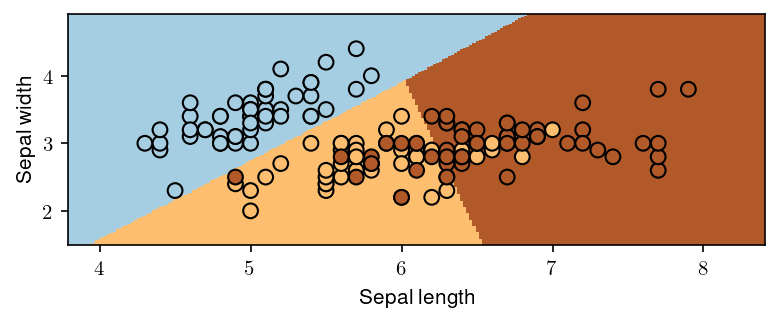
\includegraphics[width=1\textwidth]{picture_3.png}  % Ajusta el nombre y la ruta de la imagen
\end{figure}

\end{frame}


\begin{frame}[fragile]{Discriminative vs. Generative Models}


Logistic regression is an example of a \textit{discriminative} classifier.
$$
P_\theta(y| x) 
= \left[ \begin{array}{c}
P_\theta(y=0| x) \\
P_\theta(y=1| x) \\
\end{array} \right]
$$
\begin{itemize}
    \item It directly transforms $x$ into a score for each class $y$, e.g., via the formula $\sigma(\theta^\top x)$
    \item It can be interpreted as defining a *conditional* probability $P_\theta(y|x)$
\end{itemize}

Generative classifiers instead define distributions $P_\theta(x|y)$ and $P_\theta(y)$ over $x,y$.

\end{frame}


\begin{frame}[fragile]{Relation to text-to-image (TTI) models}

 \begin{itemize}
     \item TTI models can also be written as $P(x|y)$, where $x$ is an image (millions of dimensions) and $y$ is a text description of it (many possibilities).
     \item \textbf{This lecture:}  $x$ is a flower representation (4D), $y$ is a class (3 choices)
 \end{itemize}

\begin{figure}[h]
    \centering
    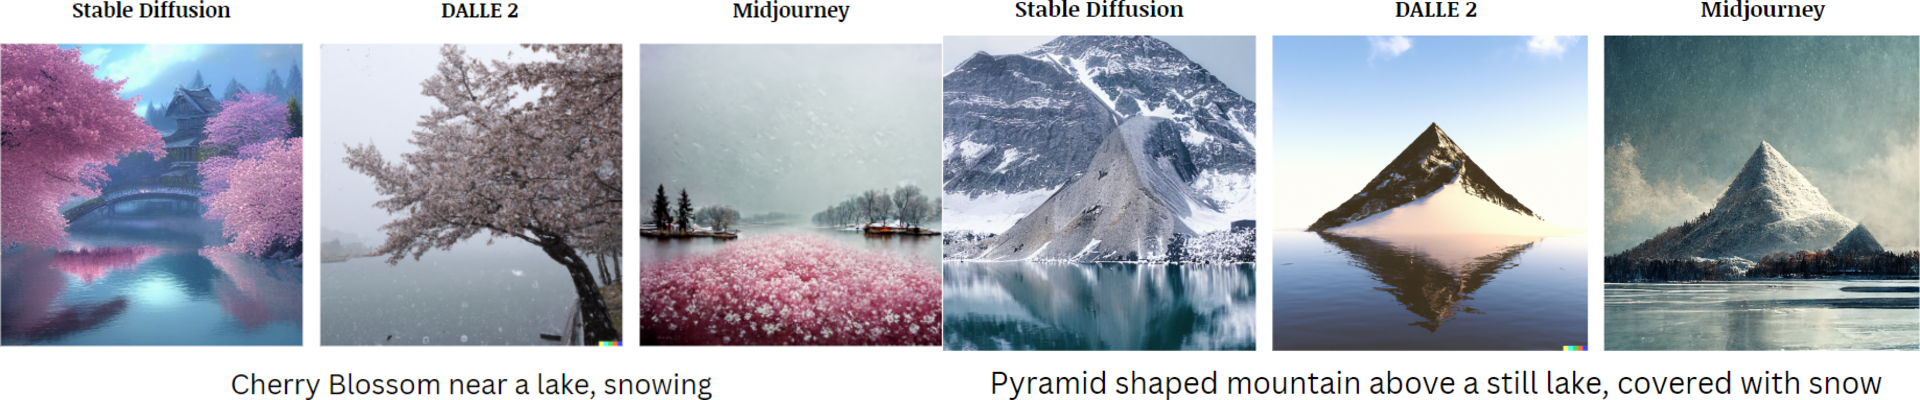
\includegraphics[width=1\textwidth]{picture_4.png}  % Ajusta el nombre y la ruta de la imagen
\end{figure}

\end{frame}


\begin{frame}[fragile]{Generative Classifiers: Intuition}

Imagine we have a dataset (e.g., flowers). We can fit a Gaussian to each class:


\begin{figure}[h]
    \centering
    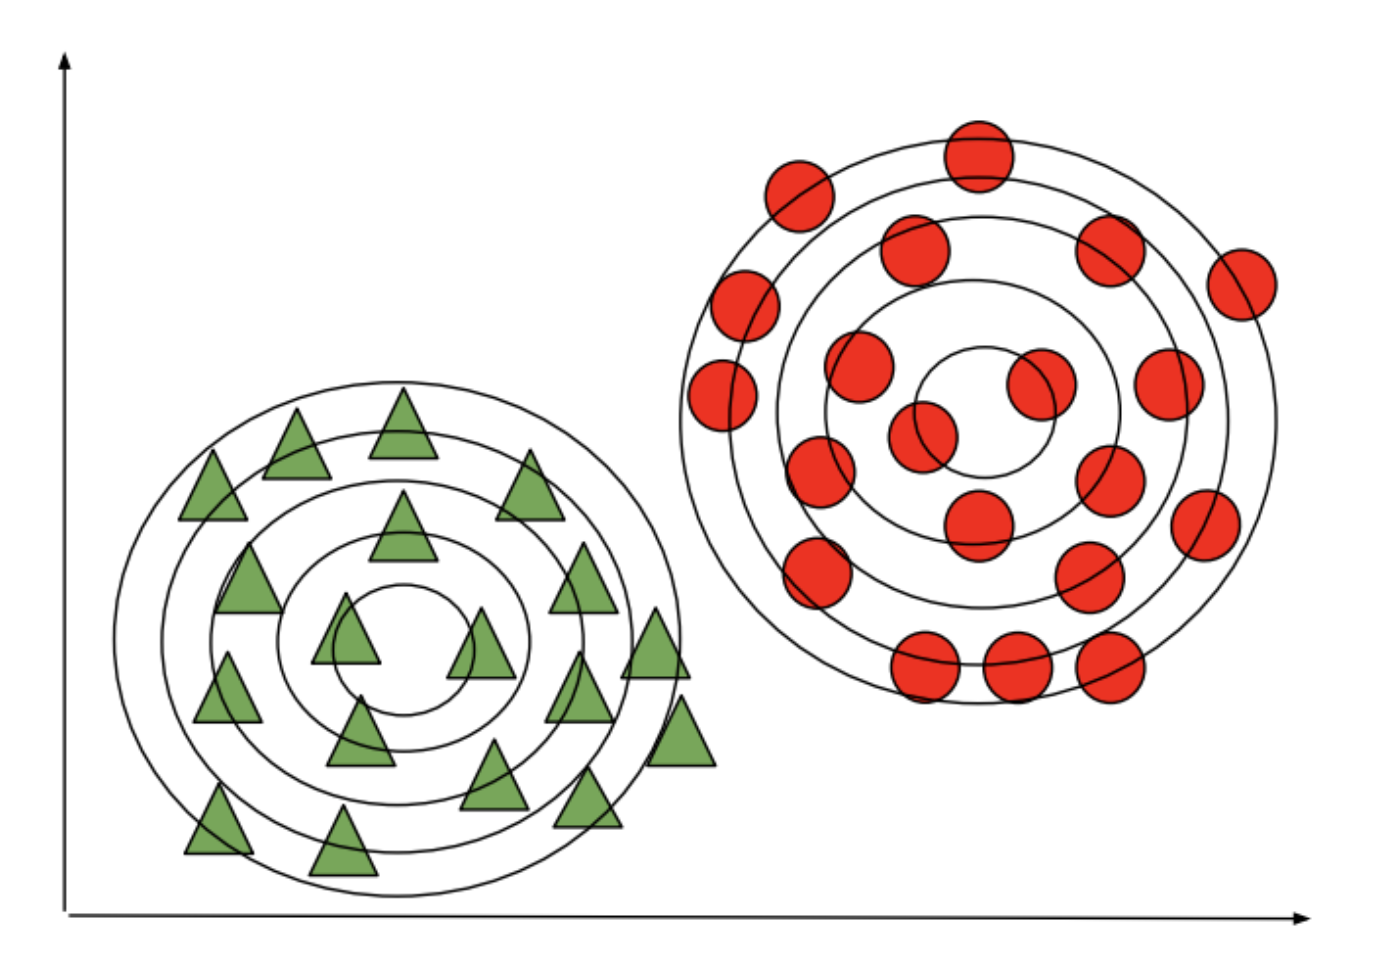
\includegraphics[width=0.5\textwidth]{picture_5.png}  % Ajusta el nombre y la ruta de la imagen
\end{figure}

At test time, we predict the class of the Gaussian that is most likely to have generated the data.


\end{frame}

\begin{frame}[fragile]{Generative Classifiers: Intuition}

Given a new flower $x'$, we would compare the probabilities of three models:

\begin{align*}
P_\theta(x'|y=\text{0})P_\theta(y=\text{0}) \\ P_\theta(x'|y=\text{1})P_\theta(y=\text{1}) \\ P_\theta(x'|y=\text{2})P_\theta(y=\text{2})
\end{align*}

We output the class that's more likely to have generated $x'$.
\end{frame}


\begin{frame}[fragile]{Generative Classifiers: Details}

Another approach to classification is to use \textit{generative} models.

\begin{itemize}
    \item A generative approach first builds a model of $x$ for each class: $$ P_\theta(x | y=k) \; \text{for each class $k$}.$$
\end{itemize}

$P_\theta(x | y=k)$ *scores* each $x$ according to how well it matches class $k$.

\begin{itemize}
    \item A class probability $P_\theta(y=k)$ encoding our prior beliefs. These are often just the \% of each class in the data.
\end{itemize}

\end{frame}

\begin{frame}[fragile]{Generative Classifiers: Details}

In the context of flower classification (e.g., Setosa vs. non-Setosa), we would fit two models on a corpus of emails $x$ with spam/non-spam labels $y$:
\begin{align*}
P_\theta(x|y=\text{0}) && \text{and} && P_\theta(x|y=\text{1})
\end{align*}

\begin{itemize}
    \item $P_\theta(x | y=1)$ \textbf{scores} each $x$ based on how much it looks like Iris Setosa.
    \item $P_\theta(x | y=0)$ \textbf{scores} each $x$ based on whether it looks like non-Setosa.
\end{itemize}
We also choose a prior $P(y)$.

Given a new $x'$, we would compare the probabilities of both models:

\begin{align*}
P_\theta(x'|y=\text{0})P_\theta(y=\text{0}) && \text{vs.} && P_\theta(x'|y=\text{1})P_\theta(y=\text{1})
\end{align*}

We output the class that's more likely to have generated $x'$.
\end{frame}

\begin{frame}[fragile]{Gaussian Mixture Models}

Next, we will define another generative model: Gaussian mixtures.

\vspace{0.3cm}

\textbf{A Generative Classifier for Iris Flowers}

To define a generative classifier for Iris flowers, we need to define three probabilities:

\begin{align*}
P_\theta(x|y=\text{0}) && P_\theta(x|y=\text{1}) && P_\theta(x|y=\text{2})
\end{align*}

We also define priors $P_\theta(y=\text{0}), P_\theta(y=\text{1}), P_\theta(y=\text{2})$.

How do we choose $P_\theta(x|y=k)$ and $P_\theta(y)$?

\end{frame}



\begin{frame}[fragile]{Review: Normal (Gaussian) Distribution}


A multivariate normal distribution with parameters $\theta = (\mu, \Sigma)$
is a probability over a $d$-dimensional $x \in \mathbb{R}^d$

$$
P_\theta(x; \mu, \Sigma) = \frac{1}{\sqrt{(2 \pi)^d | \Sigma |}} \exp\left(-\frac{1}{2} (x - \mu)^\top \Sigma^{-1} (x-\mu) \right)
$$

In one dimension, this reduces to $\frac{1}{\sqrt{2 \pi}\sigma} \exp\left(-\frac{(x - \mu)^2}{2\sigma^2} \right)$.

\vspace{0.3cm}

This is what the density of a Normal distribution looks like in 2D:

\begin{figure}[h]
    \centering
    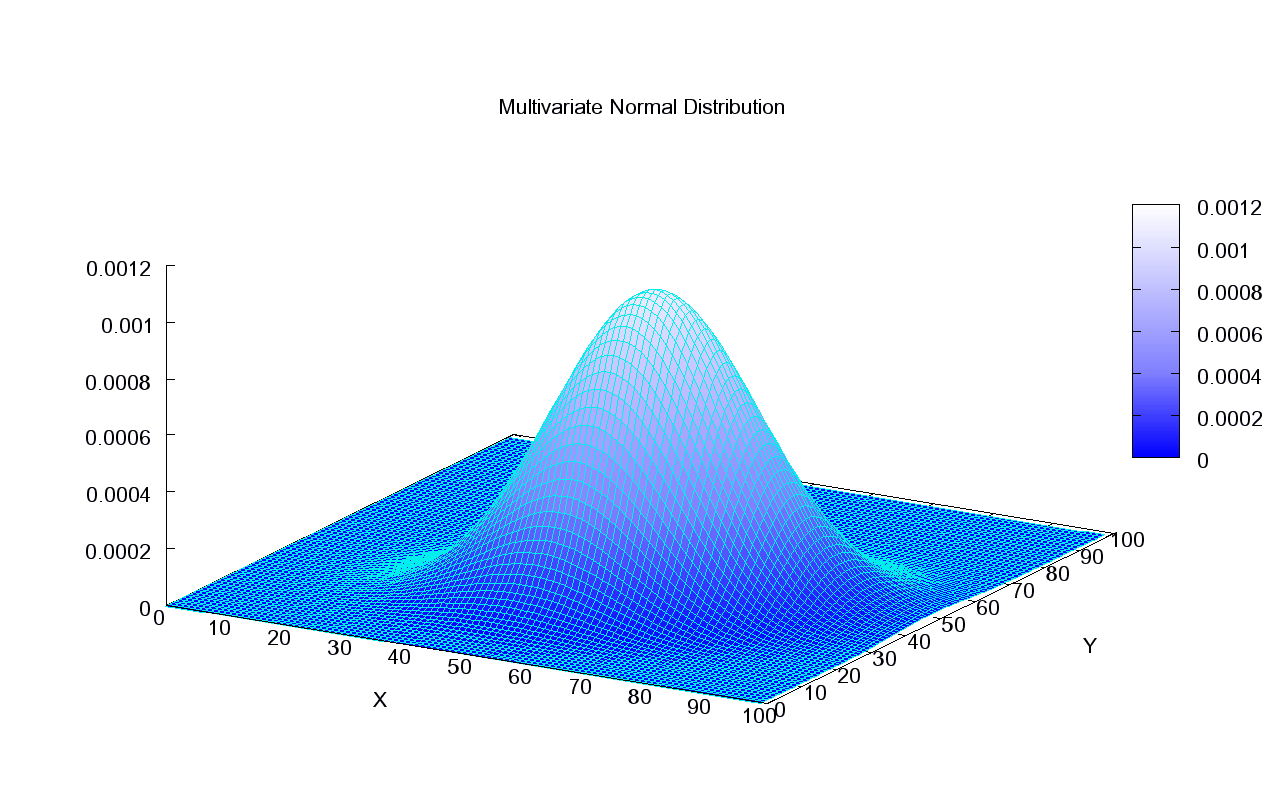
\includegraphics[width=0.45\textwidth]{multivariate_gaussian1.png}  % Ajusta el nombre y la ruta de la imagen
\end{figure}



\end{frame}

\begin{frame}[fragile]{Review: Normal (Gaussian) Distribution}


This is how we can visualize it in a 2D plane:

\begin{figure}[h]
    \centering
    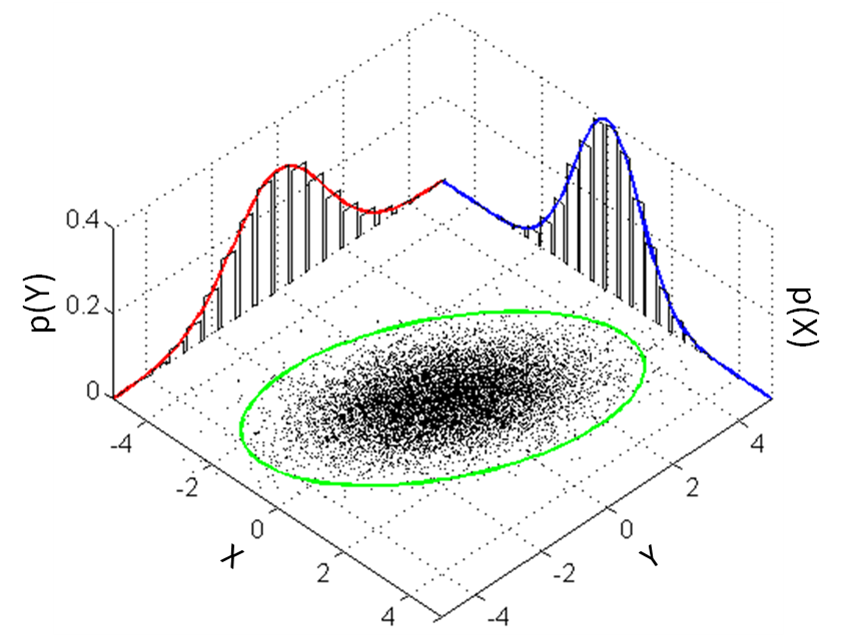
\includegraphics[width=0.63\textwidth]{multivariate_gaussian2.png}  % Ajusta el nombre y la ruta de la imagen
\end{figure}


\end{frame}

\begin{frame}[fragile]{Gaussian Mixture Model: Definition}


A \textbf{Gaussian mixture} model (GMM) $P_\theta(x,y)$ is defined for \textbf{real-valued data} $x \in \mathbb{R}^d$.

\vspace{0.3cm}
The $\theta$ contains prior parameters $\vec\phi = (\phi_1,...,\phi_K)$ and $K$ sets of per-class Gaussian parameters $\mu_k, \Sigma_k$.
\vspace{0.3cm}

The probability of the data $x$ for each class is a multivariate Gaussian
$$P_\theta(x|y=k) = \mathcal{N}(x ; \mu_k, \Sigma_k).$$

The probability over $y$ is Categorical:
$P_\theta(y=k) = \phi_k$.


\end{frame}

\begin{frame}[fragile]{Gaussian Discriminant Analysis}

Next, we will use GMMs as the basis for a new generative classification algorithm, Gaussian Discriminant Analysis (GDA).
\vspace{0.3cm}

\textbf{The Parameters of a GMM}

We need to learn the parameters of two sets of distributions:
\begin{itemize}
    \item The distribution over classes is Categorical, denoted $\text{Categorical}(\phi_1, \phi_2, ..., \phi_K)$. Thus, $P_\theta(y=k) = \phi_k$.
    \item The conditional probability $P(x\mid y=k)$ of the data under class $k$ is a multivariate Gaussian $\mathcal{N}(x; \mu_k, \Sigma_k)$ with mean and covariance $\mu_k, \Sigma_k$.
\end{itemize}

\vspace{0.3cm}
\textbf{Learning the Parameters $\mu_k, \Sigma_k$}

\begin{itemize}
    \item Consider the dataset of all the points $x$ for which $y=k$.
    \item Goal: learn the mean and variance $\theta_k=(\mu_k, \Sigma_k)$ of a Normal that generates $x$
    \item What is the maximum likelihood $\mu_k, \Sigma_k$ in this case? The formulation is: $$\arg\max_{\theta_k} P_{\theta_k}(x|y=k)$$
\end{itemize}
\end{frame}

\begin{frame}[fragile]{Gaussian Discriminant Analysis}

\begin{itemize}
    \item For Gaussians, these are the empirical means and covariances of each class.
    \begin{align*}
    \mu_k & = \frac{\sum_{i: y^{(i)} = k} x^{(i)}}{n_k} \\
    \Sigma_k & = \frac{\sum_{i: y^{(i)} = k} (x^{(i)} - \mu_k)(x^{(i)} - \mu_k)^\top}{n_k} 
    \end{align*}
\end{itemize}

\textbf{Learning the Parameters $\phi$}


Next, consider learning $\vec \phi = (\phi_1, \phi_2, \ldots, \phi_K)$. 
\begin{itemize}
    \item We have $n$ datapoints. Each point has a label $k\in\{1,2,...,K\}$.
    \item Our model is a categorical and assigns a probability $\phi_k$ to each outcome $k\in\{1,2,...,K\}$.
    \item We want to infer $\phi_k$ assuming our dataset is sampled from the model.
\end{itemize}

What are the maximum likelihood $\phi_k$ that are most likely to have generated our data?


\end{frame}

\begin{frame}[fragile]{Gaussian Discriminant Analysis}

Intuitively, the maximum likelihood class probabilities $\phi$ should just be the class proportions that we see in the data. 
$$ \phi_k = \frac{n_k}{n}$$
for each $k$, where $n_k = |\{i : y^{(i)} = k\}|$ is the number of training targets with class $k$.

Thus, the optimal $\phi_k$ is just the proportion of data points with class $k$ in the training set!
\vspace{0.3cm}

\textbf{Querying the Model}

How do we ask the model for predictions? As discussed earlier, we can apply Bayes' rule:
$$\arg\max_y P_\theta(y|x) = \arg\max_y P_\theta(x|y)P(y).$$
Thus, we can estimate the probability of $x$ and under each $P_\theta(x|y=k)P(y=k)$ and choose the class that explains the data best.


\end{frame}

\begin{frame}[fragile]{Example: Iris Flower Classification}

Let's see how this approach can be used in practice on the Iris dataset.
\begin{itemize}
    \item We will learn the maximum likelihood GDA parameters
    \item We will compare the outputs to the true predictions.
\end{itemize}

Let's first start by computing the true parameters on our dataset.

\begin{lstlisting}
# we can implement these formulas over the Iris dataset
d = 2 # number of features in our toy dataset
K = 3 # number of clases
n = X.shape[0] # size of the dataset

# these are the shapes of the parameters
mus = np.zeros([K,d])
Sigmas = np.zeros([K,d,d])
phis = np.zeros([K])

# we now compute the parameters
for k in range(3):
    X_k = X[iris_y == k]
    mus[k] = np.mean(X_k, axis=0)

\end{lstlisting}
\end{frame}

\begin{frame}[fragile]{Example: Iris Flower Classification}


\begin{lstlisting}[firstnumber=15]
    Sigmas[k] = np.cov(X_k.T)
    phis[k] = X_k.shape[0] / float(n)
\end{lstlisting}
\begin{lstlisting}
plt.scatter(X[:, 0], X[:, 1], c=Y, edgecolors='k', cmap=plt.cm.Paired, s=50);
plt.xlabel('Sepal length'); plt.ylabel('Sepal width');
\end{lstlisting}

\begin{figure}[h]
    \centering
    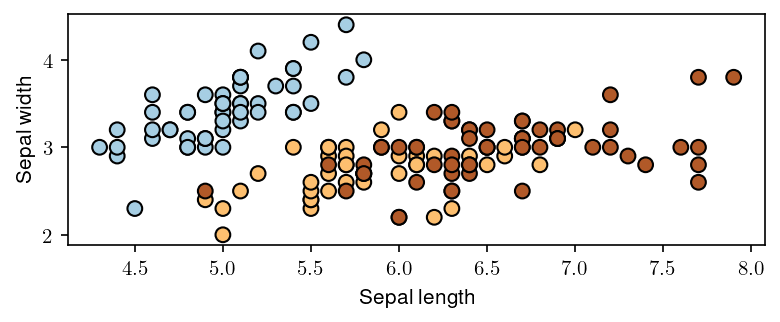
\includegraphics[width=0.8\textwidth]{picture_6.png}  % Ajusta el nombre y la ruta de la imagen
\end{figure}
\end{frame}
\begin{frame}[fragile]{Example: Iris Flower Classification}

We can compute predictions using Bayes' rule.

\begin{lstlisting}
def gda_predictions(x, mus, Sigmas, phis):
    """This returns class assignments and p(y|x) under the GDA model.
    
    We compute \arg\max_y p(y|x) as \arg\max_y p(x|y)p(y)
    """
    # adjust shapes
    n, d = x.shape
    x = np.reshape(x, (1, n, d, 1))
    mus = np.reshape(mus, (K, 1, d, 1))
    Sigmas = np.reshape(Sigmas, (K, 1, d, d))    
    
    # compute probabilities
    py = np.tile(phis.reshape((K,1)), (1,n)).reshape([K,n,1,1])
    pxy = (
   
\end{lstlisting}
\end{frame}


\begin{frame}[fragile]{Example: Iris Flower Classification}


\begin{lstlisting}[firstnumber=15] 
     np.sqrt(np.abs((2*np.pi)**d*np.linalg.det(Sigmas))).reshape((K,1,1,1)) 
        * -.5*np.exp(
            np.matmul(np.matmul((x-mus).transpose([0,1,3,2]), np.linalg.inv(Sigmas)), x-mus)
        )
    )
    pyx = pxy * py
    return pyx.argmax(axis=0).flatten(), pyx.reshape([K,n])

idx, pyx = gda_predictions(X, mus, Sigmas, phis)
print(idx)
\end{lstlisting}

\begin{figure}[h]
    \centering
    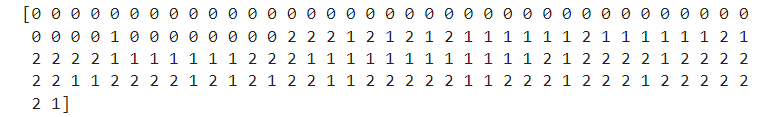
\includegraphics[width=0.8\textwidth]{picture_7.png}  % Ajusta el nombre y la ruta de la imagen
\end{figure}
\end{frame}

\begin{frame}[fragile]{Example: Iris Flower Classification}
We visualize the decision boundaries like we did earlier.

\begin{lstlisting}
Z, pyx = gda_predictions(np.c_[xx.ravel(), yy.ravel()], mus, Sigmas, phis)
logpy = np.log(-1./3*pyx)

Z = Z.reshape(xx.shape)
contours = np.zeros([K, xx.shape[0], xx.shape[1]])
for k in range(K): contours[k] = logpy[k].reshape(xx.shape)
plt.pcolormesh(xx, yy, Z, cmap=plt.cm.Paired)
for k in range(K): plt.contour(xx, yy, contours[k], levels=np.logspace(0, 1, 1))

plt.scatter(X[:, 0], X[:, 1], c=iris_y, edgecolors='k', cmap=plt.cm.Paired)
plt.xlabel('Sepal length'); plt.ylabel('Sepal width');
\end{lstlisting}


\end{frame}

\begin{frame}[fragile]{Example: Iris Flower Classification}

\begin{figure}[h]
    \centering
    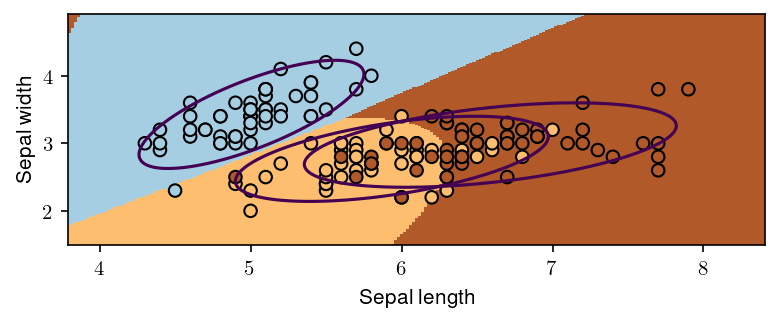
\includegraphics[width=1\textwidth]{picture_8.png}  % Ajusta el nombre y la ruta de la imagen
\end{figure}


\end{frame}


\begin{frame}[fragile]{Discriminative vs. Generative Classifiers}


We conclude our lecture on generative classifiers by revisiting the question of how they compare to discriminative classifiers.

\vspace{0.3cm}

\textbf{Linear Discriminant Analysis}

When the covariances $\Sigma_k$ in GDA are equal, we have an algorithm called Linear Discriminant Analysis or LDA.

The probability of the data $x$ for each class is a multivariate Gaussian with the same covariance $\Sigma$.
$$P_\theta(x|y=k) = \mathcal{N}(x ; \mu_k, \Sigma).$$

The probability over $y$ is Categorical:
$P_\theta(y=k) = \phi_k$.

\vspace{0.3cm}
Let's try this algorithm on the Iris flower dataset.

We compute the model parameters similarly to how we did for GDA.

\end{frame}

\begin{frame}[fragile]{Linear Discriminant Analysis}

\begin{lstlisting}
# we can implement these formulas over the Iris dataset
d = 2 # number of features in our toy dataset
K = 3 # number of clases
n = X.shape[0] # size of the dataset

# these are the shapes of the parameters
mus = np.zeros([K,d])
Sigmas = np.zeros([K,d,d])
phis = np.zeros([K])

# we now compute the parameters
for k in range(3):
    X_k = X[iris_y == k]
    mus[k] = np.mean(X_k, axis=0)
    Sigmas[k] = np.cov(X.T) # this is now X.T instead of X_k.T
    phis[k] = X_k.shape[0] / float(n)

# print out the means
print(mus)
\end{lstlisting}

\end{frame}

\begin{frame}[fragile]{Linear Discriminant Analysis}


We can compute predictions using Bayes' rule.

\begin{lstlisting}
def gda_predictions(x, mus, Sigmas, phis):
    """This returns class assignments and p(y|x) under the GDA model.
    
    We compute \arg\max_y p(y|x) as \arg\max_y p(x|y)p(y)
    """
    # adjust shapes
    n, d = x.shape
    x = np.reshape(x, (1, n, d, 1))
    mus = np.reshape(mus, (K, 1, d, 1))
    Sigmas = np.reshape(Sigmas, (K, 1, d, d))    
    
    # compute probabilities
    py = np.tile(phis.reshape((K,1)), (1,n)).reshape([K,n,1,1])
    pxy = (
        np.sqrt(np.abs((2*np.pi)**d*np.linalg.det(Sigmas))).reshape((K,1,1,1)) 
      

\end{lstlisting}
\end{frame}

\begin{frame}[fragile]{Linear Discriminant Analysis}

\begin{lstlisting}[firstnumber=16] 
  * -.5*np.exp(
            np.matmul(np.matmul((x-mus).transpose([0,1,3,2]), np.linalg.inv(Sigmas)), x-mus)
        )
    )
    pyx = pxy * py
    return pyx.argmax(axis=0).flatten(), pyx.reshape([K,n])

idx, pyx = gda_predictions(X, mus, Sigmas, phis)
print(idx)
\end{lstlisting}



\begin{figure}[h]
    \centering
    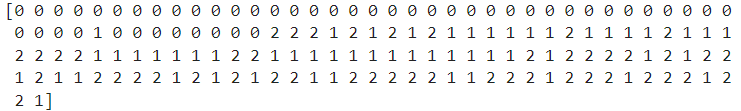
\includegraphics[width=0.8\textwidth]{picture_9.png}  % Ajusta el nombre y la ruta de la imagen
\end{figure}

\end{frame}


\begin{frame}[fragile]{Linear Discriminant Analysis}

We visualize predictions like we did earlier.

\begin{lstlisting}
Z, pyx = gda_predictions(np.c_[xx.ravel(), yy.ravel()], mus, Sigmas, phis)
logpy = np.log(-1./3*pyx)

Z = Z.reshape(xx.shape)
contours = np.zeros([K, xx.shape[0], xx.shape[1]])
for k in range(K):
    contours[k] = logpy[k].reshape(xx.shape)
plt.pcolormesh(xx, yy, Z, cmap=plt.cm.Paired)
for k in range(K):
    plt.contour(xx, yy, contours[k], levels=np.logspace(0, 1, 1))

plt.scatter(X[:, 0], X[:, 1], c=iris_y, edgecolors='k', cmap=plt.cm.Paired)
plt.xlabel('Sepal length'); plt.ylabel('Sepal width');
\end{lstlisting}

\end{frame}


\begin{frame}[fragile]{Linear Discriminant Analysis}
\begin{figure}[h]
    \centering
    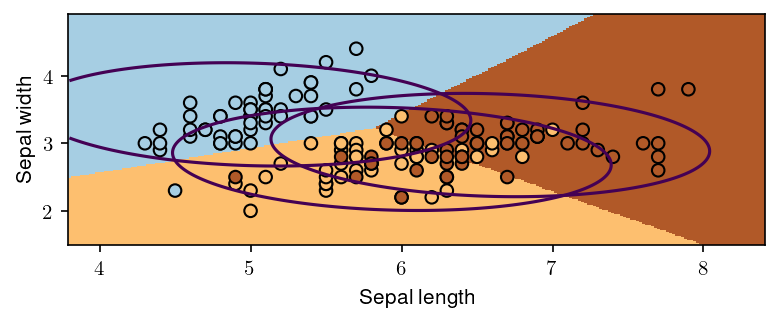
\includegraphics[width=0.75\textwidth]{picture_10.png}  % Ajusta el nombre y la ruta de la imagen
\end{figure}
Linear Discriminant Analysis outputs decision boundaries that are linear, just like Logistic/Softmax Regression.
\vspace{0.2cm}

Softmax or Logistic regression also produce linear boundaries. In fact, both types of algorithms make use of the same model class.

Are the algorithms equivalent?

\end{frame}

\begin{frame}[fragile]{What Is the LDA Model Class?}


We can derive a formula for $P_\theta(y|x)$ in a Bernoulli Naive Bayes or LDA model when $K=2$:
$$ P_\theta(y|x) = \frac{P_\theta(x|y)P_\theta(y)}{\sum_{y'\in \mathcal{Y}}P_\theta(x|y')P_\theta(y')} = \frac{1}{1+\exp(-\gamma^\top x)} $$
for some set of parameters $\gamma$ (whose expression can be derived from $\theta$). 
\vspace{0.2cm}

This is the same form as Logistic Regression! Does it mean that the two sets of algorithms are equivalent? 
\vspace{0.2cm}

No! They assume the same model class $\mathcal{M}$, they use a different objective $J$ to select a model in $\mathcal{M}$.


\end{frame}


\begin{frame}[fragile]{What Is the LDA Model Class?}


\begin{lstlisting}
nrow, ncol = 1, 2
fig, axs = plt.subplots(nrow, ncol, figsize=(6*ncol, 2*nrow))
axs[0].pcolormesh(xx, yy, Z, cmap=plt.cm.Paired); axs[0].set_title('LDA')
axs[1].pcolormesh(xx, yy, Z_lr, cmap=plt.cm.Paired); axs[1].set_title('Logistic Regression')
for ax in axs:
    ax.scatter(X[:, 0], X[:, 1], c=iris_y, edgecolors='k', cmap=plt.cm.Paired)
    ax.set_xlabel('Sepal length'); ax.set_ylabel('Sepal width')
\end{lstlisting}

\begin{figure}[h]
    \centering
    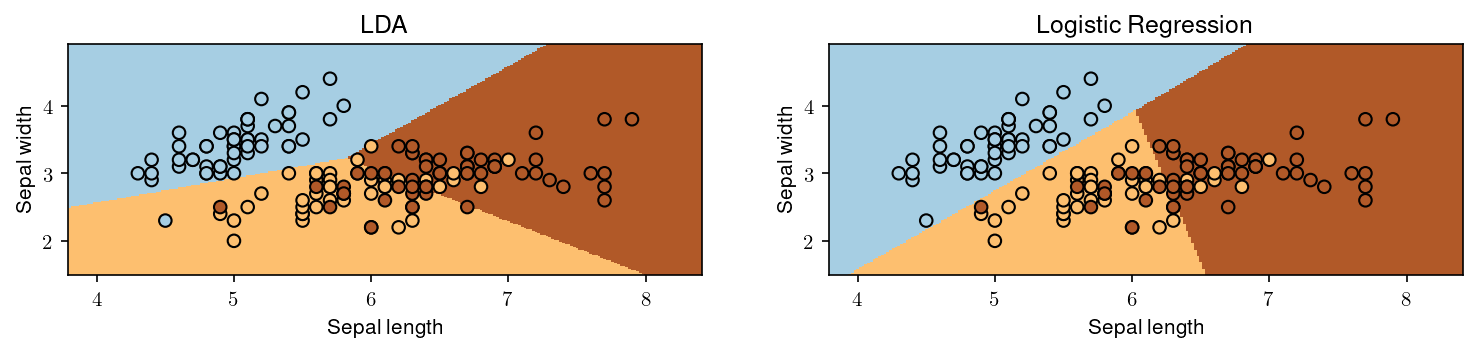
\includegraphics[width=0.9\textwidth]{picture_11.png}  % Ajusta el nombre y la ruta de la imagen
\end{figure}

\end{frame}


\begin{frame}[fragile]{LDA vs. Logistic Regression}
What are the differences between LDA/NB and logistic regression?


\begin{itemize}
    \item Bernoulli Naive Bayes or LDA assumes a logistic form for $P(y|x)$. But the converse is not true: logistic regression does not assume a NB or LDA model for $P(x,y)$.
    \item Generative models make stronger modeling assumptions. If these assumptions hold true, the generative models will perform better.
    \item But if they don't, logistic regression will be more robust to outliers and model misspecification, and achieve higher accuracy.
\end{itemize}
\vspace{0.2cm}


\textbf{Discriminative Approaches}

Discriminative algorithms are deservingly very popular.
\begin{itemize}
    \item Most state-of-the-art algorithms for classification are discriminative (including neural nets, boosting, SVMs, etc.)
    \item They are often more accurate because they make fewer modeling assumptions.
\end{itemize}



\end{frame}


\begin{frame}[fragile]{Other Useful Features of Generative Models}


Generative models can also do things that discriminative models can't do.
\begin{itemize}
    \item \textbf{Generation:} we can sample $x \sim p(x|y)$ to generate new data (images, audio).
    \item \textbf{Missing value imputation:} if $x_j$ is missing, we infer it using $p(x|y)$.
    \item \textbf{Outlier detection:} we may detect via $p(x')$ if $x'$ is an outlier.
    \item \textbf{Scalability:} Simple formulas for maximum likelihood parameters.
\end{itemize}

\end{frame}
\end{document}
